\documentclass[a4paper]{article}

%%%%%%%% CREATE DOCUMENT STRUCTURE %%%%%%%%
%% Language and font encodings
\usepackage[english]{babel}
\usepackage[utf8x]{inputenc}
\usepackage[T1]{fontenc}
%\usepackage{subfig}

%% Sets page size and margins
\usepackage[a4paper,top=3cm,bottom=2cm,left=2cm,right=2cm,marginparwidth=1.75cm]{geometry}

%% Useful packages
\usepackage{enumitem}
\usepackage{amsmath}
\usepackage{amssymb}
\usepackage{graphicx}
\usepackage[colorinlistoftodos]{todonotes}
\usepackage[colorlinks=true, allcolors=blue]{hyperref}
\usepackage{caption}
\usepackage{subcaption}
%\usepackage{sectsty}
%\usepackage{apacite}
\usepackage{float}
\usepackage{titling} 
\usepackage{blindtext}
\usepackage[square,sort,comma,numbers]{natbib}
\usepackage[colorinlistoftodos]{todonotes}
\usepackage{xcolor}
\usepackage{indentfirst}
\usepackage{amsmath}
\usepackage{mathtools}
\usepackage[linesnumbered,algoruled,boxed,lined]{algorithm2e}
\setlength\parskip{.5\baselineskip plus .1\baselineskip  minus .1\baselineskip}
\setlength{\parindent}{1em}
\definecolor{darkgreen}{rgb}{0.0, 0.4, 0.0}

\makeatletter
\def\BState{\State\hskip-\ALG@thistlm}
\makeatother

\DeclarePairedDelimiter\floor{\lfloor}{\rfloor}
\DeclarePairedDelimiter\ceil{\lceil}{\rceil}


%%%%%%%% DOCUMENT %%%%%%%%
\begin{document}



%%%% Title Page
\begin{titlepage}

\newcommand{\HRule}{\rule{\linewidth}{0.5mm}} 							% horizontal line and its thickness
\newenvironment{bottompar}{\par\vspace*{\fill}}{\clearpage}
\center 
\begin{center}
%----------------------------------------------------------------------------------------
%	HEADING SECTIONS
%----------------------------------------------------------------------------------------

\includegraphics[scale=0.8]{upclogo.png}\\[2cm] % Include a department/university logo - this will require the graphicx package
 
%\textsc{\LARGE Polytechnical University of Catalonia}\\[1cm] % Name of your university/college
\textsc{\Large Master in Innovation and Research in Informatics}\\[0.5cm] % Major heading such as course name
\textsc{\large Algorithmic Methods for Mathematical Models}\\[5cm] % Minor heading such as course title

%----------------------------------------------------------------------------------------
%	TITLE SECTION
%----------------------------------------------------------------------------------------

\HRule \\[0.4cm]
{ \huge \bfseries Solving the Nurse Scheduling Problem using Integer Linear Programming and Meta-heuristics}\\[0.4cm] % Title of your document
\HRule \\[1.5cm]
 
%----------------------------------------------------------------------------------------
%	AUTHOR SECTION
%----------------------------------------------------------------------------------------
\begin{bottompar}
\begin{minipage}{0.5\textwidth}
\begin{flushleft} \large
\emph{Authors:}\\
Adrián Rodríguez Bazaga \\ Pau Rodríguez Esmerats % Your name
\end{flushleft}
\end{minipage}
~
\begin{minipage}{0.4\textwidth}
\begin{flushright} \large
\emph{Professors:} \\
Albert Oliveras Llunel \\ Marc Ruiz Ramírez % Supervisor's Name
\end{flushright}
\end{minipage}\\[2cm]

% If you don't want a supervisor, uncomment the two lines below and remove the section above
%\Large \emph{Author:}\\
%John \textsc{Smith}\\[3cm] % Your name

%----------------------------------------------------------------------------------------
%	DATE SECTION
%----------------------------------------------------------------------------------------

{\large \today}\\[2cm] % Date, change the \today to a set date if you want to be precise
\end{bottompar}
\end{center}
\end{titlepage}

\tableofcontents
\pagebreak

\begin{abstract}
   Optimization problems can appear in almost all situations on life, but there are special important cases where those problems appears, specially on the industry, since if we can achieve an optimal solution, we will improve the efficiency of the industrial process and then get lower production cost with the same (or better) efficiency. This improvement of the costs have an effect on the competitiveness of the companies and on the final quality of their products, including that this is an important money-saving factor. 
   
   The challenging part is when this kind of problems become really big, since then they have a attached really high computational complexity and cost, therefore we need some methods to face them. 
   
   To do so, we have two approaches, the always-optimal methods that obtain the optimal solution but taking into account every possible combination of the problems' solutions, as for instance Integer Linear Programming does. By the other hand we have those methods that concerns about fair execution times and are looking for a trade-off between acceptable execution times and the quality of the solution.
   
   In this work we will propose two approaches in order to solve the scheduling of nurses in a hospital taking into account several constraints.

\end{abstract}

\pagebreak

\section{Introduction}
Optimization problems can appear in almost all situations on life, but there are special important cases where those problems appears, specially on the industry, since if we can achieve an optimal solution, we will improve the efficiency of the industrial process and then get lower production cost with the same (or better) efficiency. This improvement of the costs have an effect on the competitiveness of the companies and on the final quality of their products, including that this is an important money-saving factor. 
   
   The challenging part is when this kind of problems become really big, since then they have a attached really high computational complexity and cost, therefore we need some methods to face them. 
   
   To do so, we have two approaches, the always-optimal methods that obtain the optimal solution but taking into account every possible combination of the problems' solutions, as for instance Integer Linear Programming does. By the other hand we have those methods that concerns about fair execution times and are looking for a trade-off between acceptable execution times and the quality of the solution.
   
   In this work we propose two approaches in order to solve the scheduling of nurses in a hospital taking into account several constraints. The first one is using Integer Linear Programming and the second one by using metaheuristics. In the metaheuristics part we are focusing specifically in the Greedy Randomized Adaptative Procedure (GRASP) and the Biased-Random Key Genetic Algorithm (BRKGA).
   
   Firstly we compare the efficiency in terms of solving time and wellness of ILP and metaheuristics over medium-sized problems. 
   
   Lastly, since large problems are intractable for ILP due to combinatorial explosion reasons, we compare the metaheuristics among them to compare such kind of problems.
   
   \subsection{Problem Statement}
   
   A public hospital needs to design the working schedule of their nurses. As a first approximation, we are asked to help in designing the schedule of a single day. We know, for each hour h, that at least demandh nurses should be working at the hospital. We have available a set of nNurses nurses and we need to determine at which hours each nurse should be working. However, there are some limitations that should be taken into account:
   
   \begin{itemize}
   \item Each nurse should work at least minHours hours.
   \item Each nurse should work at most maxHours hours.
   \item Each nurse should work at most maxConsec consecutive hours.
   \item No nurse can stay at the hospital for more than maxPresence hours (e.g. if maxPresence is 7, it is OK that a nurse works at 2am and also at 8am, but it not possible that he/she works at 2am and also at 9am).
   \item No nurse can rest for more than one consecutive hour (e.g. working at 8am, resting at 9am and 10am, and working again at 11am is not allowed, since there are two consecutive resting hours).
   \end{itemize}

The goal of this project is to determine at which hours each nurse should be working in order to minimize the number of nurses required and satisfy all the aforementioned constraints.

\subsection{Document Structure}

The structure of this document is the following: The problem definition is done in chapter 2. Here it is explained the problem that is faced, which constraints is needed to take into account and what we want to optimize. At chapter 3 is explained the ILP model that has been developed, i.e. the decision variables and also the constraints with a mathematical nomenclature. After this chapter, at chapter 4 is explained how it has been used the heuristics approach in order to face with the problem, two meta-heuristics has been used: GRASP3 and BRKGA4 . After perform several executions for those approaches, a comparison in terms of time and quality of the result is done at chapter 5. Finally conclusions of the project are explained at chapter 6.

 


\pagebreak

\section{Integer Linear Programming}
Integer Linear Programming is the first of the two methods that has been used in this project (see Introduction for more details about the problem). This method always finds the optimal solution without taking into account the amount of computational
resources needed. This model is developed in CPLEX and the model implemented is described in the next sections.


\subsection{Decision variables}

\begin{itemize}

\item $ w_{n,h} (\mathbb{B})  : \text{This boolean variable specifies whether the nurse n works at the hour h (1) or not (0)}  $
\item $ z_{n} (\mathbb{B})  : \text{This boolean variable specifies whether the nurse n works during the shift or not.} $ 
	\begin{itemize}[label=$\star$]
 	\item $ z{n} = 1  \Rightarrow \text{ The nurse n works at least 1 hour, } \exists h, w_{n,h} = 1 $ 
 	\item $ z{n} = 0 \Rightarrow \forall h, w_{n,h} = 0 $ 
 	\end{itemize}
\item $  s_{n} (\mathbb{N}) : \text{Positive integer variable specifying the hour in which the nurse n starts working,} \\ \text{  such that $ w_{n,s_{n}}=1 $ and  $ w_{n,s_{n}-i}=0 $,  $ \forall i: 1 \leq s_{n} - i < s_{n} $ } $
\item $  e_{n} (\mathbb{N}) : \text{Positive integer variable specifying the hour in which the nurse n stops working,} \\ \text{such that $ w_{n,e_{n}}=1 $ and  $ w_{n,e_{n}+i}=0,\forall i : e_{n} < e_{n}+i \leq 24 $  } $
\end{itemize}

\subsection{Instance parameters}

\begin{itemize}
\item  $ demand_h $: Array of integers, specifying the required number of nurses at hour h
\item  $ nNurses $: Integer that specifies the number of available nurses to assign.
\item  $minHours$: Integer that specifies the minimum number of hours that a nurse must work if she works.
\item  $maxHours$: Integer that specifies the maximum number of hours that a nurse must work if she works.
\item  $maxConsec$: Integer that specifies the maximum number of consecutive hours that a nurse can work.
\item  $maxPresence$: Integer that specifies the maximum number of hours that a nurse can stay at the hospital.
\end{itemize}

\subsection{Objective function}
\begin{center}
Minimize $ \sum\limits_{n=1}^{nNurses} z_{n}  $ \\
\end{center}

This objective function aims to minimize the number of working nurses, this means, minimize the number of $z_n$ variables that are activated (with a value of 1), which is the main goal for our problem.

\subsection{Constraints}

\begin{itemize}
\item  Set the $z_n$ values correctly: \\ \\
\begin{equation}
 \forall n: 1 \leq n \leq nNurses,  \\
	24 \cdot z_{n}  \geq \sum\limits_{1 \leq h \leq 24} w_{n,h} \\
   z_{n} \leq \sum\limits_{1 \leq h \leq 24} w_{n,h}
 \end{equation}

\item  At any hour h, at least demandh nurses must be working: \\ \\
\begin{equation}
\forall h : 1 \leq h \leq 24, \\
 \sum\limits_{1 \leq n \leq nNurses} w_{n,h} \geq demand_{h} \\
\end{equation}

\item  Each nurse that works, must work at least minHours: \\ \\
\begin{equation}
\forall n: 1 \leq n \leq nNurses \\
	\sum\limits_{1 \leq h \leq 24} w_{n,h} \geq minHours \cdot z_{n} \\
\end{equation}

\item  Each nurse that works, must work at most maxHours: \\ \\
\begin{equation}
\forall n: 1 \leq n \leq nNurses \\
	\sum\limits_{1 \leq h \leq 24} w_{n,h} \leq maxHours \cdot z_{n} \\
\end{equation}

\item  Each nurse works at most maxConsec consecutive hours: \\ \\
\begin{equation}
\forall n:  1 \leq n \leq nNurses, \\
	\forall h_{1}:  1 \leq h_{1} \leq 24 - maxConsec, \\
	\sum\limits_{ h_{1} \leq h \leq h_{1} + maxConsec} w_{n,h} \leq maxConsec
\end{equation}

\item  Each nurse can stay in the hospital at most maxPresence hours: \\ \\
\begin{equation}
\begin{aligned}
&\forall n:  1 \leq n \leq nNurses, e_{n} \leq 24 \cdot z_{n}, \\
 &\forall n:  1 \leq n \leq nNurses, \forall h: 1 \leq h \leq 24, e_{n} \geq h \cdot w_{n,h}, \\ 
 &\forall n:  1 \leq n \leq nNurses, s_{n} \geq 0, \\
 &\forall n:  1 \leq n \leq nNurses, \forall h: 1 \leq h \leq 24, s_{n} \leq (h - 24) \cdot w_{n,h} + 24 \cdot z_{n}, \\
  &\forall n:  1 \leq n \leq nNurses: \\ &e_{n} - s_{n} + 1 - (2 \cdot 24)\cdot(1 - z_{n}) \leq maxPresence \cdot z_{n}
\end{aligned}
\end{equation}

\item  Each nurse can rest at most one consecutive hour:

\begin{equation}
\begin{aligned}
\forall n:  1 \leq n \leq nNurses, \forall h: 2 \leq h \leq 22, \forall M: M \geq 24:  \\ M - M \cdot w_{n,h-1} + M \cdot w_{n,h} + M \cdot w_{n,h+1}  \geq \sum\limits_{h+1 \leq h_{i} \leq 24 }  w_{n,h_{i}}
 \end{aligned}
\end{equation}

\end{itemize}

\pagebreak

\section{Meta-heuristics}

\subsection{GRASP implementation}

\subsubsection{Constructive phase}

The GRASP meta-heuristic has a constructive phase that is concerned to build up a feasible solution. This phase can be deterministic or include a certain amount of randomness by controlling a paremeter value $\alpha$.  This means
that for every execution, different solution could emerge. We use the basic GRASP construction phase described in \cite{grasp}. The specific parts of the implementation are the initialization of the candidate set $C$, implemented in the function $initializeCandidates$ depicted in $Algorithm$ $1$, and the greedy cost function shown in the next subsection.

\begin{algorithm}[H]
\KwIn{nNurses, hours, schedule\_constraints}
%\Parameter{Some parameter}
\KwOut{candidate list C}    

\SetKwData{Left}{left}
\SetKwData{This}{this}
\SetKwData{Up}{up}
\SetKwFunction{Union}{Union}
\SetKwFunction{FindCompress}{FindCompress}

$C$ $\leftarrow$ $\emptyset$ \\
\ForEach{$h \in hours$}{
	
	$E$ $\leftarrow$ $initializeEmptySchedules(10, hours, schedule_constraints)$ \\
	\ForEach{$hindex \in [h+1, hours]$}{ 
		$modulo\_param = 2$ \\
		\ForEach{$e \in E$}{
			\If{$hindex - h \bmod  modulo\_param > 0$}{
				addWorkingHour(e, hindex) \\
				\If{notValidConstraints(e)}{
					removeWorkingHour(e,hindex) \\
					addRestingHour(e, hindex)  \\
				}
			}
			\Else{
				addRestingHour(e, hindex) \\
				\If{notValidConstraints(e)}{
					removeRestigHour(e,hindex) \\
					addWorkingHour(e, hindex) \\
				}
			}

			\If{notValidConstraints(e, hindex - h)}{

				$E$ $\leftarrow$ $E \cap e$ \\
			}
			$modulo\_param += 1$
		}
	}
	$C$ $\leftarrow$ $C \cup E$
} 
$\textbf{return}$ <$C$>
\caption{initializeCandidates}\label{alg.mainLoop}
\end{algorithm}


The ComputeCandidateElements function takes as input the total number of nurses, the number of hours to schedule and the rest of the constraints(maximum presence hours, consecutive hours, total hours and minimum hours). The output is a list of multiple schedules that each nurse can be assigned to. A schedule is the list of hours in which a nurse works must work.\\
First, the algorithm initializes an empty candidate set. 
Then, for each hour in the schedule, it creates 10 different types of schedules beginning a this specific hour(line3). The difference between the 10 types of schedules is the compactness of the working hours. This is controlled by a parameter used to do the modulo with current hour index in the built schedule. This allows to create from the most compact schedule with all working hours consecutive until the constraints allows to do it ($hindex - h \bmod hours + 1$), to the most sparse schedule consisting of alternating working and resting hours (using $ hindex -h  \bmod 2$).
The different schedules, started at different hours are built incrementally by adding work or rest hours depending on the modulo parameter (line 7), and always taking into consideration the validity of the resulting partial schedule (line 9, 16), in which case the validity is temptatively fixed. If no more options remain and the schedule becomes invalid for the constraints of the problem(line 21), it is removed from the set $E$ (line 22) and so it is not later saved to the candidate set $C$ (line 27).

\subsubsection{Greedy cost function}

As all the nurses are equal in this scenario, there's only one thing that the greedy cost function can determine, the number of hours of demand that a single nurse schedule contributes to. We are able to do this because all schedule candidates produced are valid (they follow the constraints). We conside $e$ to be a candidate schedule for a single nurse, being $e_{h} = 1$ if the nurse has to work or 0 otherwise. We also use a big constant number K, that should be bigger than the value $hours$ (for example $nNurses$) and we consider $remaining\_demand_h$ to be the demand that is not covered by any other schedule that is present in the solution at the hour $h$	.

\begin{center}
 $ gc(e) = K - \sum_{h=1}^{Hours} remaining\_demand_h \times e_{h}$
\end{center}

\subsubsection{Other problem specific details}

There are some specific modifications of the GRASP constructie phase of \cite{grasp} applied to this problem. After updating the candidate set, in \cite{grasp} page 2, we test the feasibility of the updated solution in each iteration of the constructive phase, and in the case we are having a feasible solution, we leave the loop. If not, we continue looping until no candidate schedules are available or no more candidate schedules can be added (all nurses have a schedule). A solution is feasible if for each hour, the demand is less or equal to the number of nurses working at this hour. Another improvement introduced in the basic version of the algorithm, is the fact that instead of removing candidate elements(single nurse schedules) from the candidate set and adding them to the solution, we generate a basic list of possible candidates and each time a nurse is assigned one of them, we don't remove it from the candidate set. What we do is recompute each time the greedy cost of each candidate when the solution is updated. This is possible thanks to the fact that all nurses are equal under the problem assumptions and constraints. That way we reduce the number of candidates that we have to generate and sort.



\subsubsection{Local Search}

The other part that will be shown is about the local search. Once the constructive phase ends up with a solution, eventually it is the optimal, but usually it is not. In order to improve the solution a neighbourhoods of the constructive phase solution, i.e. near solutions will be searched. This phase is called local search. You can see the pseudocode 4.1.3 for the implemented local search procedure.

In the intensive Local Search ($Algorithm$ $3$) we take as input an incumbent solution, the max number of failed iterations for this Local Search procedure and finally the parameters of the problem instance (number of nurses, number of hours, demand per hour). As output a solution is returned.

The procedure starts by initializing the number of failed iterations ($failedIterations$) to 0 (line 1). Now we iterate while the number of failed iterations is less than the number of max failed iterations (line 2). Inside the loop, we start by calculating an auxiliary solution by applying a first improvement local search over the incumbent solution (line 3). We check if the used nurses (objective function of the problem) of the auxiliary solution we have just got from the first improvement local search is greater or equal than the  used nurses by the incumbent solution (line 4), this means that the intensified solution is of the same quality or worse than the previous solution, so in this case we have failed to intensify the solution and get a better one, so the failed iterations counter is increased by 1 (line 5). Otherwise we successfully got a better solution by intensification so the failed iterations counter is reinitialized to 0. At the end of the loop, the incumbent solution is replaced by the auxiliary solution found (line 11) and returned as solution (line 12).

\begin{algorithm}[H]
\KwIn{incumbentSolution, maxFailedIterations, nNurses, hours, demand}
%\Parameter{Some parameter}
\KwOut{solution}    

\SetKwData{Left}{left}
\SetKwData{This}{this}
\SetKwData{Up}{up}
\SetKwFunction{Union}{Union}
\SetKwFunction{FindCompress}{FindCompress}

failedIterations $\leftarrow$ 0 \\
\While{$failedIterations$ $<$ $maxFailedIterations$}{
solution' $\leftarrow$ firstImprovementLocalSearch(incumbentSolution, nNurses, hours, demand) \\
\If{getUsedNurses(solution') $\geq$ getUsedNurses(incumbentSolution)}{\label{lt}
failedIterations += 1
}
\Else{failedIterations = 0}{\label{lt}
}
}
incumbentSolution $\leftarrow$ solution'\\
$\textbf{return}$ incumbentSolution
\caption{Intensive Local Search}\label{alg.mainLoop}
\end{algorithm}

\begin{algorithm}[H]
\KwIn{solution, nNurses, hours, demand}
%\Parameter{Some parameter}
\KwOut{solution}    

\SetKwData{Left}{left}
\SetKwData{This}{this}
\SetKwData{Up}{up}
\SetKwFunction{Union}{Union}
\SetKwFunction{FindCompress}{FindCompress}
solution' $\leftarrow$ solution \\
computeExceedingNurseHours(solution', nNurses, hours, demand) \\
exceedingCapacityRemoval(solution', nNurses, hours, demand) \\
improved $\leftarrow$ $\textbf{TRUE}$ \\
\While{$improved$}{
improved $\leftarrow$ $\textbf{FALSE}$ \\
findRestschedules(solution, nNurses, hours, demand) \\
\ForEach{$n$ $\in$ $nNurses$}{\label{lt}
solution' $\leftarrow$ exchangeWorkingHours(n) \\
\If{isNotFeasible(solution', nNurses, hours, demand)}{\label{lt}
$\textbf{break}$
}
\ElseIf{getUsedNurses(solution') $<$ getUsedNurses(solution)}{\label{lt}
improved $\leftarrow$ $\textbf{TRUE}$ \\
}
}
}
solution $\leftarrow$ solution'\\
$\textbf{return}$ solution
\caption{First Improvement Local Search}\label{alg.mainLoop}
\end{algorithm}




\subsection{BRKGA implementation}

\subsubsection{Chromosome structure}

For this implementation, the chromosome will encode the order in which the hours are tried to be fulfilled with nurses. The decoder is behaving as a greedy algorithm but with some modification in order to work with the chromosome as you will see at X. Then the chromosome will have as many gens as hours, and every gen will have a value from 0 to 1. This value is the weight that modify the order of the fulfilled hours at the decoder.



\subsubsection{Decoder}

Recapping, the greedy algorithm is based on the idea to bring for every candidate a value that depicts the quality of every of them. This value is provided by the greedy function. For purely greedy algorithms, the candidates are sorted by this value and then the best one (the first one of the list) will be included on the solution. An evolution of greedy is GRASP that is randomizing the pick of a candidate with its RCL. This decoder is following the same idea, but taking as order the one given my the chromosome structure, being this order the priority of hours to fulfill.

This means that the gens are affecting to the position of the hours to fulfill in the assignment phase. Once we have all the hours sorted, the first one is picked. Notice that the decoder is deterministic. The randomness in BRKGA is not in the greedy part but in the generation of mutants



\pagebreak

\section{Testing, Tunning and Comparisons}
\subsection{Benchmarking instances}

This section explains the two sets of benchmarks used for testing the ILP, GRASP and BRKGA models. First we discuss about how the size of a problem instance can be determined. Then we show how we created two sets of problems instances, the medium size data set consisting of 38 small or medium size instances, and the large size data set consisting of 200 problem instances. The medium size set is used to compare the ILP model versus the Metaheuristics models. The large size set is used to test parameter values in order to find the best performing setup for each BRKGA and GRASP model, and finally to compare them solving one large problem instance.


\subsubsection{The instance generation process}

The algorithm used for generate problem instances is based on generating random but valid schedules of nurses and then extracting the demand for each schedule. This approach assures that the problem instance will always have a solution.

The algorithm takes as input: the number of nurses, the proportion of extra nurses to add to the minimum needed to solve the problem, the hours of the schedule and the rest of the constraints of the schedules (max hours, min hours, max presence and max consecutive hours). It then generates 2 types of schedules, one that concentrates the working hours as much as the constraints allow it to, and another one with as much alternated rest hours and working hours as the constraints permit it. Then the algorithm can choose to place the generated schedules around selected hours (the algorithm can choose one, two, three or four different hours to start working schedules at). We add some variability on the exact hour at which each schedule starts around the selected hours. Once all schedules are placed, the number of working nurses for each our is added and the demand for each hour is then computed.


\subsubsection{The medium and large sets}

To decide how the size of a problem is determined, we choose to reference the time it takes for the ILP model to solve the problem instance using the Cplex solver. We generate and solve a series of instances with the ILP until we have around 20 instances that take 60 minutes or less to solve by ILP. Then, as we cannot perform the same procedure to generate the large size set, we execute a series of experiments to determine the influence of the problem variables in the time it takes for the ILP model to solve it.\\

The next figures show different executions of a small modification of a problem instance. In each figure, a parameter of the problem is modified to increase the time it takes to the ILP model to solve the instance problem. This gives us an idea of what parameters increase the size of the problem instance.\\


\begin{figure}[h!]

\begin{subfigure}[b]{.49\linewidth}
\centering
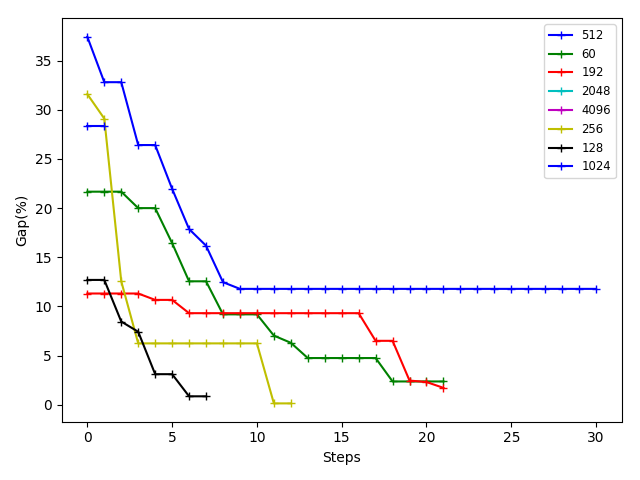
\includegraphics[width=\linewidth]{./img/instances_nurses_ilp_evol.png}
\caption{ Evolution of Gap of the ILP model with different number of nurses}\label{fig1a}
\end{subfigure}%
\begin{subfigure}[b]{.49\linewidth}
\centering
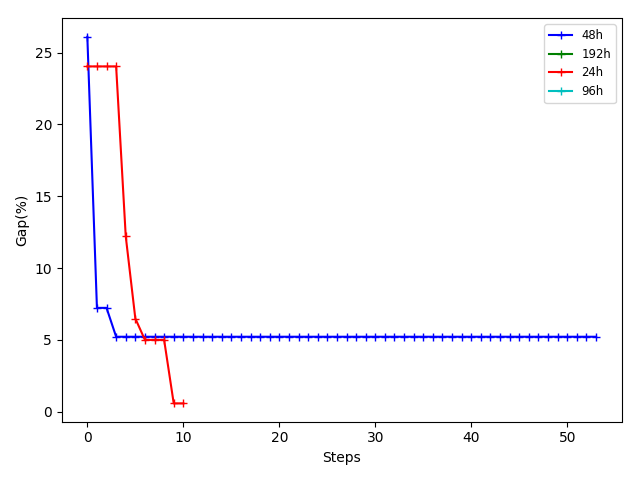
\includegraphics[width=\linewidth]{./img/instances_hours_ilp_evol.png}
\caption{ Evolution of Gap of the ILP model with different number of hours }\label{fig1b}
\end{subfigure}\vfill
\caption{Evolution of Gap of the ILP model with different values of number of nurses (\subref{fig1a}) and number of hours (\subref{fig1b}). }
\label{fig_ilp_size}
\end{figure}


\begin{figure}[h!]
\begin{subfigure}[b]{.49\linewidth}
\centering
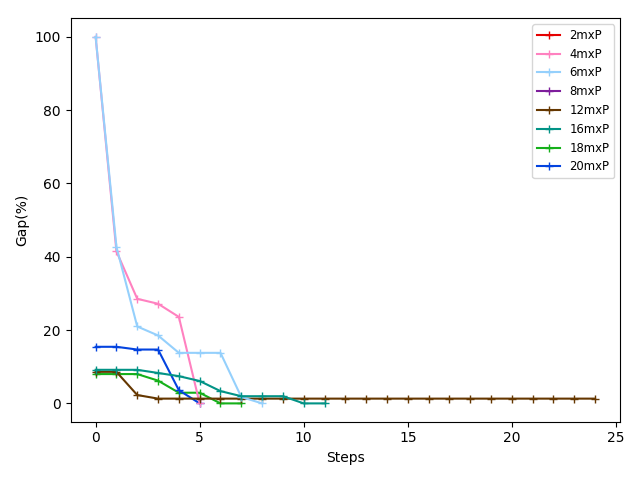
\includegraphics[width=\linewidth]{./img/instances_maxpresence_ilp_evol.png}
\caption{Evolution of Gap of the ILP model with different values of maxPresence parameter }\label{fig1c}
\end{subfigure}
\begin{subfigure}[b]{.49\linewidth}
\centering
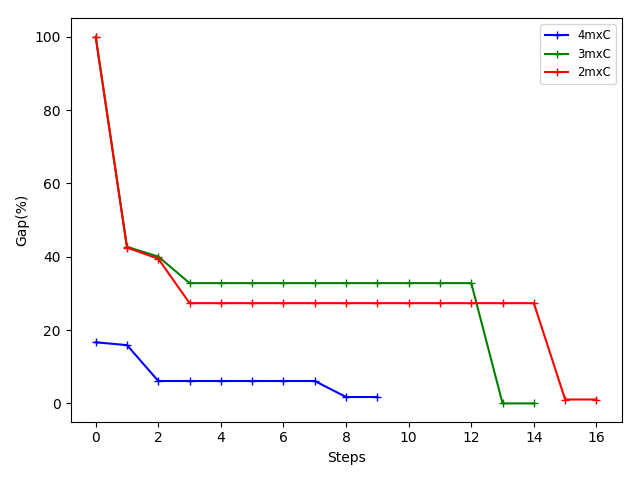
\includegraphics[width=\linewidth]{./img/instances_maxconsec_ilp_evol.png}
\caption{Evolution of Gap of the ILP model with different values of maxConsec parameter }\label{fig1d}
\end{subfigure}
\caption{Evolution of Gap of the ILP model with different values of maxPresence (\subref{fig1c}) and maxConsec (\subref{fig1d}).  }
\label{fig_ilp_size2}
\end{figure}


\begin{figure}[h!]
\begin{subfigure}[b]{.49\linewidth}
\centering
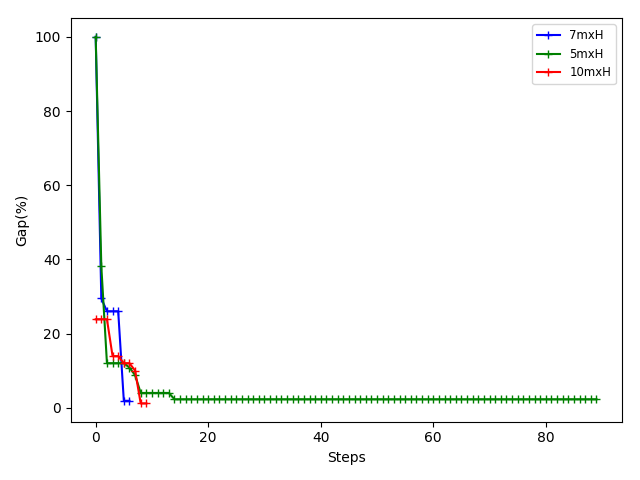
\includegraphics[width=\linewidth]{./img/instances_maxhours_ilp_evol.png}
\caption{Evolution of Gap of the ILP model with different values of maxHours parameter }\label{fig1c}
\end{subfigure}
\begin{subfigure}[b]{.49\linewidth}
\centering
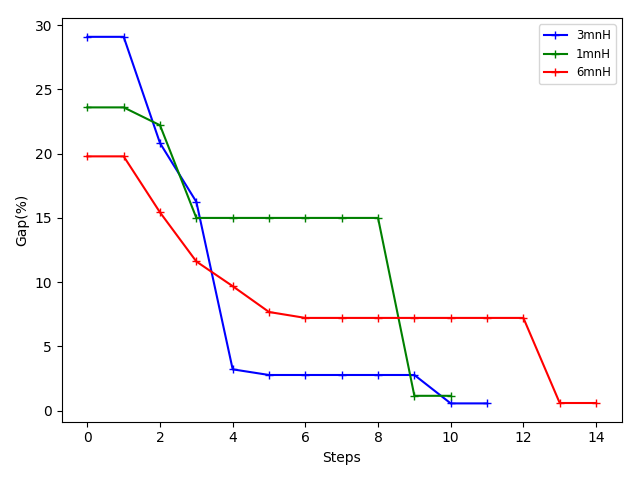
\includegraphics[width=\linewidth]{./img/instances_minhours_ilp_evol.png}
\caption{Evolution of Gap of the ILP model with different values of minHours parameter }\label{fig1d}
\end{subfigure}
\caption{Evolution of Gap of the ILP model with different values of maxHours (\subref{fig1c}) and minHours (\subref{fig1d}).  }
\label{fig_ilp_size3}
\end{figure}


The results in figure~\ref{fig_ilp_size}, figure~\ref{fig_ilp_size2} and figure~\ref{fig_ilp_size3} allow us to conclude how the parameters of the problem instance can be modified to increase its solving time and thus what we consider its size. The large set of problem instances will be generated using modifications of those instance variables, applied to some problems of the medium size set. The table~\ref{tab:ilp_size} page~\pageref{tab:ilp_size} summarizes the findings and shows the attributes of each benchmark instance set.

\begin{table}[ht] 
\centering 
\begin{tabularx}{0.75\textwidth}{|l|c|c|c|}
\hline
\textbf{Problem} & \textbf{Effect on problem size}  & \textbf{Medium size set} & \textbf{Large size set} \\

\textbf{Variable}  		& \textbf{when increasing}  & 38 instances &  199 instances \\
\hline
\textbf{$nNurses$} & increases      &  64	&  64 to 1600 \\
\textbf{$hour$}   & increases		& 24	&  24, 48, 72 \\
\textbf{$maxPrensce$} & decreases	& 16	& 8 to 27 \\
\textbf{$maxConsec$} & decreases		& 5	&  4 to 13		\\
\textbf{$maxHours$} & decreases		& 4 to 10	& 2 to 12 \\
\textbf{$minHours$} & increases		& 1 to 5	& 1 to 9\\
\hline
\end{tabularx}
\caption{Benchmark datasets and variables influence on problem size}
\label{tab:ilp_size}
\end{table}




\subsection{Comparing Integer Linear Programing to Meta-heuristics}

In this section, we are going to compare the execution results of the Cplex ILP solver and the two metaheuristics algorithms. We are going to solve the problem instances of the medium size data set with our three solvers and plot the results in terms of solving time and objective function. All executions have been performed on the same computer. The parameters for the BRGKA and GRASP algorithms are respectively kept with the same values during all executions. For this experiment, the size of the problems will be determined by the time it takes the ILP solver to find the optimal solution.\\


\begin{figure}[h!]

\begin{subfigure}[b]{.49\linewidth}
\centering
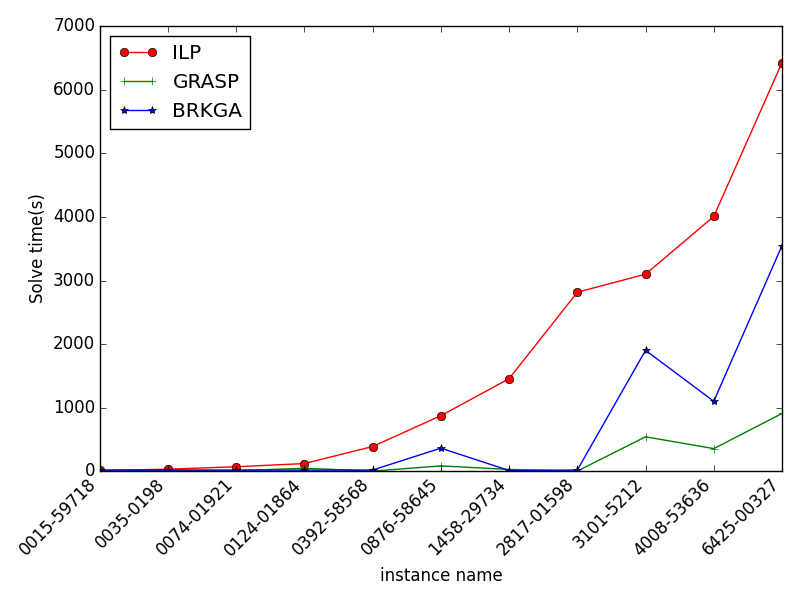
\includegraphics[width=\linewidth]{./img/ILPvsMetah_times.png}
\caption{ Solving times for 38 instances of the mediume set}\label{fig1a}
\end{subfigure}%
\begin{subfigure}[b]{.49\linewidth}
\centering
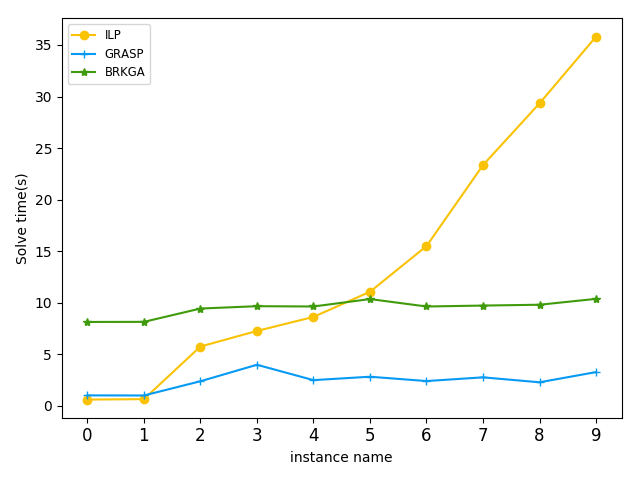
\includegraphics[width=\linewidth]{./img/ILPvsMetah_times_first10.png}
\caption{ Solving times for the first 10 instances }\label{fig1b}
\end{subfigure}\vfill
\begin{subfigure}[b]{.49\linewidth}
\centering

\includegraphics[width=\linewidth]{./img/ILPvsMetah_objf_hist.png}
\caption{Objective function values for 38 instances of the medium set }\label{fig1c}
\end{subfigure}
\begin{subfigure}[b]{.49\linewidth}
\centering
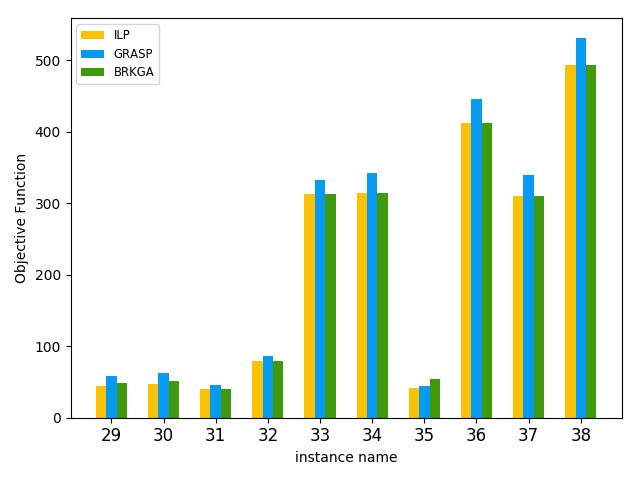
\includegraphics[width=\linewidth]{./img/ILPvsMetah_objf_hist_last10.png}
\caption{Objective function values for the last 10 instances  }\label{fig1d}
\end{subfigure}
\caption{Solving times in seconds (\subref{fig1a}, \subref{fig1b}) and objective function values (\subref{fig1c}, \subref{fig1d}) for the instances of the medium size set solved by ILP, GRASP and BRKGA.  }
\label{fig_ilp_vs_meta}
\end{figure}


The figure~\ref{fig_ilp_vs_meta} on page~\pageref{fig_ilp_vs_meta}, shows that the ILP execution times increase exponentially as the size of the problem instance increases, whereas the GRASP and BRKGA solving times increase much more slowly.
We observe that for the bigger instances, the GRASP algorithm produces worse results (bigger objective function values), whereas the BRKGA produces results very close to the optimum objective function found by the ILP solver.

\pagebreak

\subsection{Comparison of GRASP and BRKGA models}

Test of the section: parameter selection for each model, model performance comparision with best parameter setup.


\subsubsection{GRASP parameter selection}


Setup of the tests:\\
\begin{itemize}
	\item instances set
	\item execution conditions (same computer)
	\item procedure
	\item results and times gathering procedure
\end{itemize}


Graph of alpha\\
Graph of Iterations\\
Graph of best improvement vs first improvement?\\

\subsubsection{BRKGA parameter selection}


Setup of the tests:\\
\begin{itemize}
	\item instances set
	\item execution conditions (same computer)
	\item procedure
	\item results and times gathering procedure
\end{itemize}


Graph of iheritance probability\\
Graph of elite proportion\\
Graph of mutant proportion\\
Graph of population size\\
Graph of number of generations\\

\subsubsection{Metaheuristic models comparision}

Choosing the best performing parameter setup of the two models, perform a comparison of how objective function evolves in relation to time.

Draw conclusions about, why one is better than the other, why one stops sooner than the other. (think in terms of diversification and intensification and solution space exploration)\\

\pagebreak

\section{Conclusions}
The conclusion may contain facts discovered throught the comparision of solving times. Thoughs about intensification and diversification of the algorithms. Parametrizations that work and why the do, etc..


\pagebreak

\appendix
\section{Appendices}
\thispagestyle{empty}
\subsection{Running the launcher}

To solve instances of the problem with the models run, from ./Tools/Launcher:

For ILP (calls oplrun from commandline) python launcher.py --solver ILP

For GRASP python launcher.py --solver grasp For BRKGA

python launcher.py --solver brkga

These commands solve all instances from the default folder ./Instances/Pending and save the results in a json format to ./Results/Pending Options:

Instances folder and results folder (paths must be relative to ./Tools/Launcher) : python launcher.py --solver grasp --instances ../../Instances/Final/MediumSet --results ../../Results/Final/MediumSet

GRASP parameters: python launcher.py --solver grasp --iterations 5 --alpha 0.15 --ls best

BRKGA parameters: python launcher.py --solver brkga --generations 1 --eliteprop 0.3 --mutantprop 0.2 --population 2 --inheritance 0.1 --decoder <hini,horder,hexcess>

\subsection{Parameter validation (LargeSet)}

$ cd Tools/Launcher python megalauncher_grasp.py ../../Instances/Final/LargeSet_20180106/$

Quick demo of the files and dirs created in ../../Results/Final/LargeSet\_20180103/. It does not execute any solver, just time.sleep(0.5) cd Tools/Launcher python megalauncher.py --demo ../../Instances/Final/LargeSet

Real execution cd Tools/Launcher python megalauncher.py ../../Instances/Final/LargeSet See results in ../../Results/Final/LargeSet\_20180103/ See progress files in ../../Results/Progress/

\subsubsection{Other options}

Other options that can be used are to use the ./Metaheuristics/main.py file from it's 'main' section, calling any of the "entry points" of the Metaheuristics algorithms.

\subsection{Reporting}

mediumSetGraph.py, takes all json files in a folder and creates 2 graphs, one comparing the solving times for differents instances for the 3 algorithms (ILP, GRASP and BRKGA). It expects to find json files with results from executions of the 3 algorithms in the indicated folder: python mediumSetGraph.py ../../Results/MediumSet

summary\_of\_executions.py, example file that reads json results files from a folder and plots all the resutls in a graph

classifier.py script used to organize the executions of instances by the ILP, it saves the instances files (.dat) to the Instances/Final/ with a name that reflects the time it takes for the ILP to solve it.

\end{document}